\documentclass[12pt]{amsart}
\pagestyle{empty}
\usepackage[hmargin=1in,vmargin=1in]{geometry}
\usepackage{url,  mathrsfs}
\usepackage{hyperref}
\usepackage{fancyhdr} 
\usepackage{amssymb} 
\usepackage{tikz}
\usepackage[T1]{fontenc}


\usepackage{url,  mathrsfs}
\usepackage{hyperref}
\usepackage{amsmath}
\usepackage{graphicx,  epstopdf}
\usepackage{subfig}
\usepackage{color}
\usepackage{bbm}
\usepackage{subfloat}
\usepackage[draft]{fixme}
\usepackage{bm} 
\usepackage{bbm} 
\usepackage{epigraph}
\usepackage{endnotes}
\usepackage{ifpdf}
\usepackage{array}

\usepackage{multicol}
\usepackage{multirow}
\usepackage{graphicx}
\usepackage{tikz}

\newcommand{\A}{\mathbb{A}}
\newcommand{\Q}{\mathbb{Q}}
\newcommand{\N}{\mathbb{N}}
\newcommand{\Z}{\mathbb{Z}}
\newcommand{\R}{\mathbb{R}}
\newcommand{\F}{\mathbb{F}}
\newcommand{\C}{\mathbb{C}}
\renewcommand{\P}{\mathbb{P}}
\newcommand{\I}{\mathcal{I}}
\newcommand{\V}{\mathcal{V}}
\newcommand{\cH}{\mathcal{H}}
\newcommand{\ol}{\overline}
\newcommand{\J}{\mathcal{J}}
\newcommand{\X}{\mathcal{X}}
\theoremstyle{definition}
\newtheorem{prob}{Problem}
\newtheorem{extraProb}{Extra Problem}

\DeclareMathOperator{\conv}{conv}
\DeclareMathOperator{\cone}{cone}
\DeclareMathOperator{\ext}{ext}

\usepackage{listings,xcolor}
\lstset{language=Mathematica}
\lstset{basicstyle={\sffamily\footnotesize},
  numbers=left,
  numberstyle=\tiny\color{gray},
  numbersep=5pt,
  breaklines=true,
  captionpos={t},
  frame={lines},
  rulecolor=\color{black},
  framerule=0.5pt,
  columns=flexible,
  tabsize=2
}

\begin{document}
 \thispagestyle{empty}
\begin{center} {\large \textbf{Math 380 -- Homework  1}} \smallskip \\ 
Due on Thursday, April 9\ \\ \ \\
 \end{center}

You are welcome to talk with other students in the class about problems but should write up solutions on your own. 
Solutions can be handwritten or typed but need to be legible and submitted via Gradescope by the end of the day 
on Thursday. You should justify all your answers in order to receive full credit.  
\bigskip 

\begin{flushleft}

{\bf Good practice problems} (not to be turned in): \\
CLO Section 1.1, Exercises 2, 6\\
CLO Section 1.2, Exercises 4, 13, 15\\
CLO Section 1.3, Exercises 1, 4, 8\\
\bigskip 




\begin{prob} CLO \S1.2, Exercise 6 and 
\begin{itemize}
\item[a.] A point $(a_1,\dots,a_n) \in k^n$ is an affine variety. Consider the variety $V(x_1 - a_1, \dots, x_n - a_n)$. We have a system of $n$ equations, and we must have that for all $1 \le i \le n$, $x_i - a_i = 0$, implying that $x_i = a_i$ for all $i$. Thus, $(a_1,\dots,a_n)$ is the only solution to the system, and it is the only point in our variety.
\item[b.] Every finite subset $A \subseteq k^n$ is an affine variety. Let $|A|=m$, and perform induction starting from $m=0$. In this case, $A=\varnothing=V(1)$ is a variety. Consider the inductive case for $m>0$, and let $a \in A$ be any element. Then $A \setminus \{a\}$ is a finite subset of $k^n$ with cardinality $m-1$, so by the inductive hypothesis it as an affine variety. In part (a), we have shown that single points are affine varieties, so $\{a\}$ is an affine variety. Thus, we can write $A$ as the union of two affine varieties, $(A\setminus \{a\})\cup \{a\}$. By Proposition 2, the union of two varieties is a variety, so $A$ is an affine variety.
\item[c.] The set $\{(0,0), (1,0), (0,1)\}$ can be written as an affine variety in $\R^2$:
\begin{align*}
    V(xy, x(x-1),y(y-1))
\end{align*}
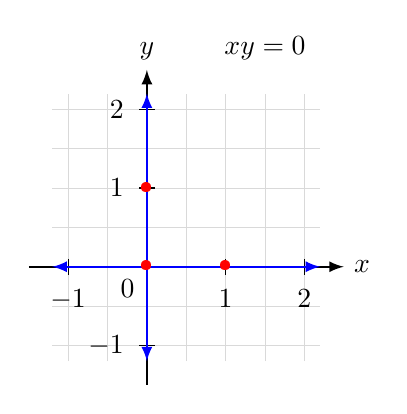
\begin{tikzpicture}[>=latex]
    \draw[step=0.5cm, gray!30, very thin] (-1.2, -1.2) grid (2.2, 2.2);
    \draw[thick, ->] (-1.5, 0) -- (2.5, 0) node[right] {$x$};
    \draw[thick, ->] (0, -1.5) -- (0, 2.5) node[above] {$y$};
    \draw (1.5,2.5) node[above] {$xy=0$};
    \foreach \x in {-1, 1, 2} {
        \draw (\x, 0.1) -- (\x, -0.1) node[below=2pt] {$\x$};
    }
    \foreach \y in {-1, 1, 2} {
        \draw (0.1, \y) -- (-0.1, \y) node[left=2pt] {$\y$};
    }
    \node[below left=1pt] at (0,0) {$0$};
    \draw[blue,thick, <->] (-1.2, 0) -- (2.2, 0);
    \draw[blue,thick, <->] (0, -1.2) -- (0, 2.2);
    \foreach \p in {(0,0), (1,0), (0,1)} {
        \node[red] at \p {\textbullet};
    }
\end{tikzpicture}
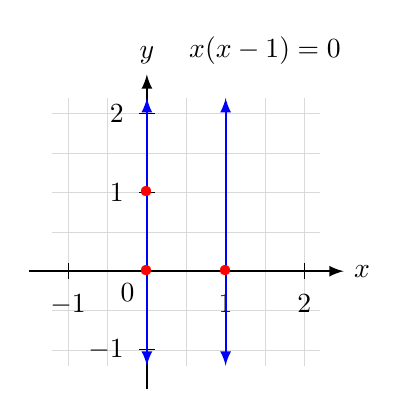
\begin{tikzpicture}[>=latex]
    \draw[step=0.5cm, gray!30, very thin] (-1.2, -1.2) grid (2.2, 2.2);
    \draw[thick, ->] (-1.5, 0) -- (2.5, 0) node[right] {$x$};
    \draw[thick, ->] (0, -1.5) -- (0, 2.5) node[above] {$y$};
    \draw (1.5,2.5) node[above] {$x(x-1)=0$};
    \foreach \x in {-1, 1, 2} {
        \draw (\x, 0.1) -- (\x, -0.1) node[below=2pt] {$\x$};
    }
    \foreach \y in {-1, 1, 2} {
        \draw (0.1, \y) -- (-0.1, \y) node[left=2pt] {$\y$};
    }
    \node[below left=1pt] at (0,0) {$0$};
    \draw[blue,thick, <->] (1, -1.2) -- (1, 2.2);
    \draw[blue,thick, <->] (0, -1.2) -- (0, 2.2);
    \foreach \p in {(0,0), (1,0), (0,1)} {
        \node[red] at \p {\textbullet};
    }
\end{tikzpicture}
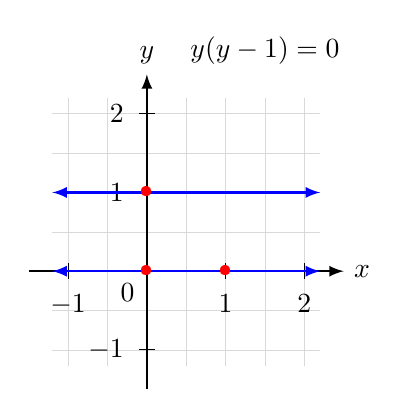
\begin{tikzpicture}[>=latex]
    \draw[step=0.5cm, gray!30, very thin] (-1.2, -1.2) grid (2.2, 2.2);
    \draw[thick, ->] (-1.5, 0) -- (2.5, 0) node[right] {$x$};
    \draw[thick, ->] (0, -1.5) -- (0, 2.5) node[above] {$y$};
    \draw (1.5,2.5) node[above] {$y(y-1)=0$};
    \foreach \x in {-1, 1, 2} {
        \draw (\x, 0.1) -- (\x, -0.1) node[below=2pt] {$\x$};
    }
    \foreach \y in {-1, 1, 2} {
        \draw (0.1, \y) -- (-0.1, \y) node[left=2pt] {$\y$};
    }
    \node[below left=1pt] at (0,0) {$0$};
    \draw[blue,thick, <->] (-1.2, 1) -- (2.2, 1);
    \draw[blue,thick, <->] (-1.2, 0) -- (2.2, 0);
    \foreach \p in {(0,0), (1,0), (0,1)} {
        \node[red] at \p {\textbullet};
    }
\end{tikzpicture}\\ 
\[(x = 0 \lor y=0)\land (x=0\lor x=1)\lor (y=0\lor y=1).\]
More explanation here?
\end{itemize}
\end{prob}
\bigskip 

\newpage{}
\begin{prob} CLO \S1.2, Exercise 8

The set 
\[ X = \{(x,x) \mid x \in \mathbb R, x \ne 1\} \subseteq \mathbb R^2 \]
is not an affine variety. Assume FTSOC that $X = V(f_1, \dots, f_s)$. Then, every polynomial $f_i$ must vanish on $X$. However, we prove that any polynomial $f \in \mathbb R[x,y]$ that vanishes on $X$ also vanishes on $(1,1)$, leading us to derive $(1,1)\in X$, a contradiction. Let $g \in \mathbb R[x]$ be given by $g(x)=f(x,x)$. Because $f$ must vanish on $X$, this $g$ must vanish on $\mathbb R \setminus \{1\}$. Since $g$ has infinitely many distinct roots, $g$ must be the zero polynomial as any nonzero polynomial must have a finite degree $d$ and at most $d$ distinct roots. We can then evaluate $g(1)=0=f(1,1)$, so any variety that contains $X$ must also contain $(1,1)$. $X$ is not an affine variety.
\end{prob}
\bigskip 

\begin{prob} CLO \S1.3, Exercise 6 and 
\begin{itemize}
\item[a.] A rational parametrization of the sphere can be constructed by projecting all points onto the plane $z=0$ using the line passing through the north pole $(0,0,1)$. This takes the southern hemisphere to the unit disk and the northern hemisphere to the complement of the unit disk. The north pole itself goes to the point at infinity but we don't worry about that... See \ref{fig:placeholder} and appendix for code.
\begin{figure}
    \centering
    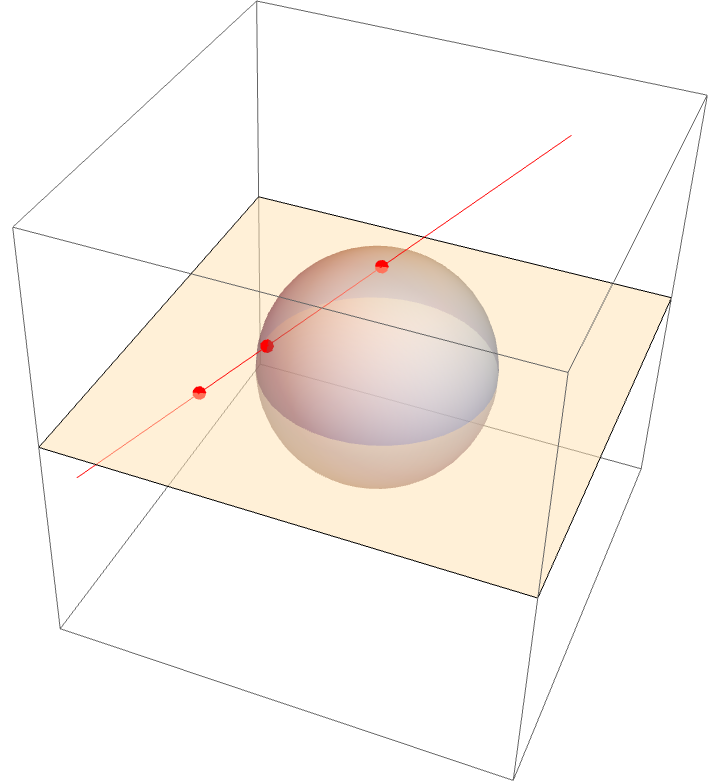
\includegraphics[width=0.5\linewidth]{math380hw1.png}
    \caption{The projection used to construct the rational parametrization of $\mathbb S^2$.}
    \label{fig:placeholder}
\end{figure}
\item[b.] The line passing through $(0,0,1)$ and $(u,v,0)$ can be written $\vec r(t) = \begin{bmatrix}0\\0\\1\end{bmatrix} + \left( \begin{bmatrix}u\\v\\0\end{bmatrix} -\begin{bmatrix}0\\0\\1\end{bmatrix} \right)t$ so that $\vec r(0)$ and $\vec r(1)$ lands on the desired points. Thus, the line is parameterized by $(ut,vt,1-t)$.
\item[c.] Solving for where this line intersects $\mathbb S^2$, we substitute into $x^2 +y^2+z^2 = 1$:
\begin{align*}u^2 t^2 + v^2 t^2 +(1-t)^2 &= 1 \\
t^2(u^2 + v^2+1)+1-2t&=1 \\
\qquad t([u^2 +v^2 +1]t-2)&=0.
\end{align*}
We take the nonzero solution of $t=\frac{2}{u^2 + v^2 + 1}$. Substituting this value of $t$ into the equation for the line, we get
\begin{align*}
    x &= u t = \frac{2u}{u^2 + v^2 + 1} \\
    y &= v t = \frac{2v}{u^2 + v^2 + 1} \\
    z &= 1 - t = 1 - \frac{2}{u^2 + v^2 + 1} = \frac{u^2 + v^2-1}{u^2 + v^2 + 1}.
\end{align*}
\item[d.] We can use this parametrization to generate Pythagorean quadruples, \emph{i.e.} positive integers $a, b, c, d\in \Z_{>0}$ for which $a^2+b^2+c^2=d^2$. Take $a = 2u$, $b = 2v$, $c = u^2 + v^2 - 1$, and $d=u^2 + v^2 + 1$ for $u,v \in \mathbb Z_{>0}$. Taking $u=2$ and $v=3$, we get $4^2 + 6^2 +12^2 = 14^2$.
\end{itemize}
\end{prob}
\bigskip 

\section{Appendix - Mathematica Code}
\begin{lstlisting}[language=Mathematica]
Manipulate[
 Graphics3D[
  With[{u = pt[[1]], v = pt[[2]], 
    d = pt[[1]]^2 + pt[[2]]^2 + 1}, {Opacity[0.5], Sphere[], 
    InfinitePlane[{{0, 0, 0}, {1, 0, 0}, {0, 1, 0}}], Opacity[1], Red,
     PointSize[0.02], Point[{0, 0, 1}], Point[{u, v, 0}], 
    Point[{2 u/d, 2 v/d, (u^2 + v^2 - 1)/d}], 
    InfiniteLine[{{0, 0, 1}, {u, v, 0}}]}], 
  PlotRange -> {{-2, 2}, {-2, 2}, {-2, 2}}], {pt, {-2, -2}, {2, 2}}]
\end{lstlisting}
\end{flushleft}
\end{document}